\documentclass{article}
\usepackage{amsmath, amsfonts, amsthm} % Math packages

\usepackage{listings} % Code listings, with syntax highlighting

\usepackage[english]{babel} % English language hyphenation

\usepackage{graphicx} % Required for inserting images

\usepackage{geometry} % Required for adjusting page dimensions and margins
\usepackage{indentfirst}

\geometry{
	paper=a4paper, % Paper size, change to letterpaper for US letter size
	top=2cm, % Top margin
	bottom=2cm, % Bottom margin
	left=3cm, % Left margin
	right=3cm, % Right margin
	headheight=0.75cm, % Header height
	footskip=1.5cm, % Space from the bottom margin to the baseline of the footer
	headsep=0.75cm, % Space from the top margin to the baseline of the header
	%showframe, % Uncomment to show how the type block is set on the page
}

\title{	
	\normalfont\normalsize
	\textsc{ Physics 5CL}\ % Your university, school and/or department name(s)
	\vspace{25pt} % Whitespace
	\rule{\linewidth}{0.5pt}\ % Thin top horizontal rule
	{\huge A Study of Planck’s Law and Blackbody Radiation}\ % The assignment title
	\rule{\linewidth}{2pt}\ % Thick bottom horizontal rule
}

\author{\LARGE Daniel Geisz \& Heidi Hu} % Your name

\date{\normalsize\today}

\begin{document}
\maketitle 
\section{Objectives} % (fold)
\label{sec:objectives}	
For our capstone project, we wish to test Planck’s Law for the Blackbody Radiation spectrum.  Planck's Law takes the form:

$$B_\lambda (\lambda, T) = \frac{2hc^2}{\lambda ^5}\frac{1}{e _{}^{\frac{hc}{\lambda k_B T} - 1}}$$

Here, $B_{\lambda}$ is the spectral radiance of Blackbody, $\displaystyle h$, $c$, and $k_B$ are Planck's unreduced constant, the speed of light, and Boltzmann's Constant respectively, and $T$ and $\lambda$ are the temperature of Blackbody and the wavelength of light respectively.


In this lab, we will measure the temperature of an approximate blackbody and the luminosity of light emitted from the approximate blackbody at different wavelengths.   By varying the temperature of the blackbody, we can find the wavelength at which the luminosity is greatest for a given temperature. Once we have done this, we can use Wien's Law:

$$\lambda_{max} = \frac{b}{T}$$

to experimentally determine Wien's Constant $b$.  Wien's Constant theoretically takes the form:

$$b = \frac{hc}{xk_B}$$

where $x$ is the solution to the equation:

$$\frac{xe^x}{e^x - 1} - 5 = 0$$

which can be numerically solved to yield:

$$x \approx 4.965114231744276$$

If we take $k_B$ and $c$ as given, we can therefore use our experimentally determined value of $b$ to experimentally determine Planck's unreduced constant.
 
% section objectives (end)

\section{Equipment} % (fold)
\label{sec:equipment}
\begin{itemize}
	\item Photodetector \& Computer with corresponding software (like in Lab 2)
\item	Tungsten Lightbulb
\item	DC Power supply.  If possible, this power supply should give us voltage and current readings
\item	Multimeter
\item	Diffraction Grating with the highest possible Slit Density
\item	Optical Bench Stands
\item	Ruler \& Meterstick
\item	Opaque Box with a slit (To place over the Tungsten Bulb)
\item	Optical Pyrometer, or some other device that can be used to measure the temperature of the bulb.  If the lab does not have access to this type of sensor, we can use a different method to determine the temperature of the lightbulb, but it will be less accurate.

\end{itemize}

\section{Experimental Setup and Procedure:} % (fold)
\label{sec:experimental_setup_and_procedure_}

Refer to Figure 1 for the Experimental Setup.
Note that the Power Source in the figure should be a DC power supply because we need to vary the voltage across the bulb in order to vary the temperature of the bulb.  

\subsection{Procedure:} % (fold)
\label{sub:procedure_}
\begin{enumerate}
	\item Measure the temperature of the Tungsten Bulb
	\begin{enumerate}
		\item We will either do this by directly measuring the temperature of the bulb with an optical pyrometer, or we will use the equation for the Temperature Dependence of Resistivity by measuring the resistance of the bulb using the Power Supply readings or multimeter.
	\end{enumerate}
	\item	Measure the luminosity of the light emitted at different wavelengths
	\begin{enumerate}
		\item To do this, we will keep the aperture of the photodetector at a constant distance from the diffraction grating, and by measuring the luminosity of the light emitted at different angles, we use a measurement the angle between the photodetector and the vector normal to the grating to find the luminosity of the light emitted at different wavelengths. 
	\end{enumerate}
	\item	Repeat steps 1 and 2 for different temperatures of the Tungsten Bulb
	\begin{enumerate}
		\item By varying the voltage across to the Tungsten Bulb, we can change the temperature of the filament inside the bulb.
	\end{enumerate}
\end{enumerate}


% subsection procedure_ (end)
\begin{figure}
  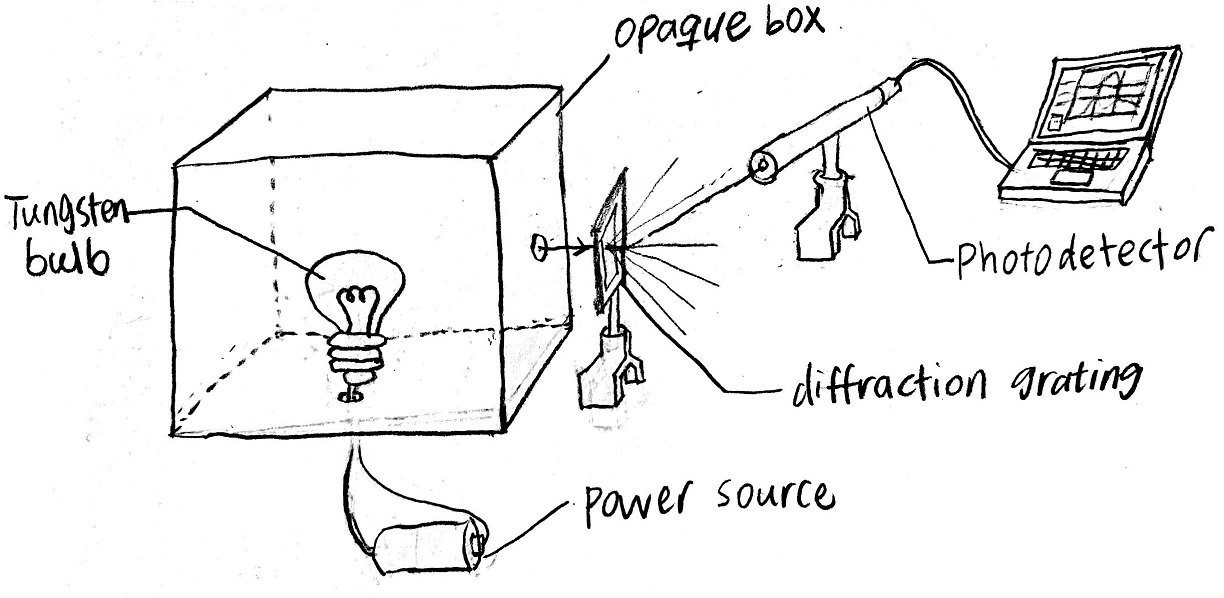
\includegraphics[width=10cm]{IMG-0011.jpg}
  \caption{Capstone Setup}
  \label{fig:boat1}
\end{figure}

\section{Expected Outcome:} % (fold)
\label{sec:expected_outcome_}
Once we finish the lab work, we should have data for the spectral luminosity of a tungsten bulb at different temperatures.  If we can accurately calculate the effective area of the aperture of the photodetector, we can then find the spectral radiance of the tungsten bulb at different temperatures.  Either way, we can use our data to find the wavelength at which the luminosity or radiance of light emitted reaches a maximum for a given temperature, and we can use this data to calculate Wien’s constant and Planck’s unreduced constant.   We can also use our data to show that blackbody radiation behaves according to Planck’s law, and contradicts classical theory (The Ultraviolet Catastrophe).
% section expected_outcome_ (end)
% section experimental_setup_and_procedure_ (end)
% section equipment (end)
\end{document}